\chapter{The Large Hadron Collider}\label{thelhc}
%
%
The Large Hadron Collider (LHC) is the world's largest particle accelerator, designed to store and accelerate proton and \lead beams at unprecedented energies of 7$\,Z\,$TeV. The LHC is a synchrotron of 26.7\,km length, installed in the underground tunnel of the former Large Electron Positron Collider (LEP) at the CERN\footnote{Centre Europ\'{e}en pour la Recherche Nucl\'{e}aire} research center in proximity to Geneva, Switzerland. With the Relativistic Heavy-Ion Collider (RHIC) at the Brookhaven National Laboratory in Long Island (USA), it is one of the two heavy-ion colliders ever built and operated\cite{Fischer2014}. In the first operational period (LHC run 1), the LHC reached energies up to 4$\,Z\,$TeV and collected an integrated luminosity of 29.2\,fb$^{-1}$~\cite{lamont_moyab101} with proton beams and xx.x\,fb$^{-1}$ with \lead beams. With the collected data, the discovery of the long sought Higgs Boson could be announced in July 2012~\cite{higgs:ATLAS,higgs:CMS}. After a phase of machine and detector upgrades from 2013 to 2015, the LHC re-started and accelerated proton beams to the unprecedented energy of $6.5\,$TeV and \lead beams to $6.37\,Z\,$TeV.
%

In this chapter the LHC is presented with the sub-systems relevant for the development of the heavy-ion collimation simulations presented later-on. Particular emphasis is given to the LHC collimation system and the physics processes relevant for heavy-ion collimation.

%
\section{The CERN Accelerator Complex}
%
  \begin{figure}[t]
    \centering
    \includegraphics[width=0.85\textwidth]{pictures/14052201.png}
    \caption{ The CERN Accelerator Complex~\cite{Christiane:1260465}.}  
    \label{pic:14052201}
  \end{figure}
%
The LHC is a high energy synchrotron operated at the end of a complex chain of injectors which pre-accelerate and prepare the beam for its requirements. The ensemble of accelerators which is presently in operation at CERN, referred to as the CERN accelerator complex, is schematially illustrated in Fig.~\ref{pic:14052201}. 

The LHC injector chain originates from two different ion sources, respectively delivering proton or heavy-ion beams. The generation of proton beam starts at a hydrogen ion source feeding the linear accelerator LINAC2, in which the proton beam is accelerated to a momentum of 50~MeV\footnote{For clarity, in this chapter the momementum is given in natural units. All given momenta shall correspond to the correct unit of eV$/c$. Furthermore, the energies for the non fully stripped ions are given in terms of momentum per nucleon, while for the fully stripped ions, the general convention of using the momentum per charge is followed.} and injected in to the Proton Synchrotron Booster. This synchrotron accelerates the beam to 1.4~GeV, the injection energy of the Proton Synchrotron (PS) which provides acceleration up to 25~GeV. After the subsequent injection into the Super Proton Sychrotron (SPS), the beams are brought to 450~GeV, the injection energy of the LHC~\citedr. 
%

Heavy-ion beams originate from the ion source which is connected upstream of the linear accelerator LINAC3. The ions are generated from a block of isotopically pure Pb$^{208}$ by means of an Electron Cyclotron Resonance Source~\cite{CERN-2004-003-V1}. The source delivers ions at a momentum of 2.5\,keV/$A$, which are sent to a spectrometer in order to extract the desired Pb$^{+27}$ charge state. After the filtering, a multi-stage RF system accelerates the selected ion species to a momentum of $4.2\,$MeV/$A$. The following 300~nm thick stripper foil removes more electrons, such that an ion beam of Pb$^{+53}$ is extracted from LINAC3 and transferred to the circular accelerator LEIR (Low Energy Ion Ring). In the latter, the ion beams are cooled, e.g. the transverse emittance is reduced by an adiabatic process using electron scattering. In parallel, the beam is accelerated to a momentum of 72$\,$keV$/A$ at which it is extracted and transferred into the PS. In this machine, the ions bunches are re-shaped and accelerated to a momentum of 5.9$\,$GeV$/A$ and sent to the SPS. Another stripper foil in the transfer line between PS and SPS removes the remaining electrons, such that the ion arriving at the SPS is \lead. The SPS provides the acceleration to the energy of $450\,Z\,$GeV at which the beams are injected into the LHC~\citedr.


\section{LHC Layout}
\subsection{Global Layout}
%
\figref{pic:15032201} shows the LHC layout with its eight straigt insertion regions (IR), four of which host the main experiments (IR1, IR2, IR5 and IR8). The remaining four IRs provide operational functionalities, in particular betatron and momentum cleaning in IR3 and IR7 (see ~\chapref{chap:3}), acceleration in IR4 and the beam dump in IR6. The straight sections are seperated by eight arc regions, in which the particle beams are transported from IR to IR by means of a periodic array of 1232 superconducting dipole magnets and 392 superconducting quadrupole magnets. 
%
%
\begin{figure}[b]
  \centering
  \includegraphics[width=0.7\textwidth]{pictures/15092509.pdf}
  \caption{The layout of the LHC. Based upon \cite{Bruning2012705,CERN-2004-003-V1}.}  
  \label{pic:15032201}
  %/home/phermes/Dropbox/codes/latex/150305_eps2pgf/test.pdf
\end{figure}


\subsection{Insertion Region Layout and Optics}

%IR should be explained in previous section

Each element of the LHC is associated with a cell number, indicating the number of quadrupoles between the closest IP and the respective location. For example the name MQY.4L5.B1 denotes a quadrupole of the MQY type (see \cite{CERN-2004-003-V1}) in cell 4 left of IP5 for Beam 1. 
%
\begin{figure}[b]  
    \centering
    \includegraphics[width=0.9\textwidth]{pictures/16051203.pdf}
    \caption{Optical functions at the experimental insertion IR5 with $\beta^*=1\,$m for a flat machine (no seperation or crossing bump).}  
    \label{pic:16051202}
    %/home/phermes/Dropbox/PhD/pictures/160403_optics/IR5.pdf
\end{figure}
%
The schematic layout of the experimental insertion regions is shown together with the $\beta$ functions in \figref{pic:16051202}. Downstream of the main arcs (1) in which the beams are transported between the IRs, the dispersion suppressor (DS) region (2) serves the purpose of reducing the periodic dispersion function. This is reached by means of a missing dipole structure, in which one of three dipoles is omitted, compared to the nominal dipole structure in the arcs~\citedr. In between the surrounding DS regions, the IR is free of the main dipoles and therefore straight. After the DS, the matching section (3) adjusts the $\beta$ functions to the requirements of the following sections. The separation/recombination dipoles (4) and (5) guide the beams from the separated beam pipes into a common beam pipe. The superconducting triplet magnets (6) provide the final focusing for the experiment at the interaction point (7) (IP) where the beams are brought into collision.

The experiments ATLAS and CMS demand for the highest possible luminosity in order to gain enough statistics for the study of rare processes (see \chapref{chap:lumi}). As discussed later, the luminosity is inversely proportional to the $\beta$ value at the IP (denoted as $\beta^*$), thus the optical lattice is optimized to minimize the $\beta^*$ value. Following Liouville's theorem, small $\beta$ functions imply a large divergence (large $\alpha$ function) at the IP and, due to the absence of magnets between IP and triplet, the $\beta$ functions (and associated with it the beam size) at the superconducting triplets increase with smaller $\beta^*$. The normalized dimensions of the triplet aperture therefore impose a lower limit on the achievable $\beta^*$. This includes effects of adiabatic damping, such that the transition to the smallest $\beta^*$ settings (referred to as squeeze) is performed either at top energy or at the end of the energy ramp (see \chapref{chap:lhccycle}). At injection energy, the optics in IR1 and IR5 are set to $\beta^*=11\,$m while IP2 and IP8 are set to $\beta^*=10\,$m. A summary of the $\beta^*$ values achieved at top energy during the past LHC runs is given in \tabref{tab:betastar}. 
%
%
\begin{table}[htbp]
\centering
\caption{Minimum $\beta^*$ values in LHC operation compared to the design values.}
\label{tab:betastar}
\begin{tabular}{ccccc}
Configuration & Species & \begin{tabular}[c]{@{}c@{}}$\beta^*$\\
IP1/IP5 {[}m{]}\end{tabular} & \begin{tabular}[c]{@{}c@{}}$\beta^*$\\
IP2 {[}m{]}\end{tabular} & \begin{tabular}[c]{@{}c@{}}$\beta^*$\\ IP8
{[}m{]}\end{tabular} \\ \toprule
%
Design & $p$ & 0.55 & 10.0 & 10.0 \\
2011 & $p$ & 1.0 & 10.0 & 3.0     \\
2012 & $p$ & 0.6 & 10.0 & 3.0     \\
2015 & $p$ & 0.8 & 10.0 & 3.0     \\
2016 & $p$ & 0.4 & 10.0 & 3.0     \\ \midrule
Design & Pb & 0.5 & 0.5 & 10.0    \\
2011 & Pb & 1.0 & 1.0 & 3.0       \\
2013 & $p$-Pb & 0.8 & 0.8 & 2.0   \\
2015 & Pb & 0.8 & 0.8 & 3.0       \\ \bottomrule
%
\end{tabular}
\end{table}
%
% table: proton and ion runs, beta*


In the central part of the experimental insertions both beams are moving in a common vacuum pipe to allow for bringing the beams into collision. In order to avoid unwanted collisions of the counter-rotating beams, a seperation bump is applied at every time collisions are not supposed to occur. Furthermore, even when the beams are brought into collision, a crossing bump avoids secondary collisions at parasitic bunch encounters.  The crossing and seperation bumps are, except in IR8, orthogonal to each other. Both bumps are shown for the example of IR5 in \figref{pic:16051204}.

% The closed orbit in the experimental insertions is in general at the center of the beam pipe. Exceptions are  In these regions, the beam orbits are not in the center of the beam pipe to avoid unwanted collisions of the counter-rotating beams. A seperation bump is applied during all phases except when the beams should collide in the IP. The seperation bump is collapsed to establish collisions~\citedr. 

% Depending on the bunch spacing, multiple encounters of the two counter-rotating beams may be localized in the common beam pipe. The application of a crossing bump prevents from parasitic collisions at these secondary bunch encounters.

The functional IRs are not equipped with triplet magnets and the optics is adjusted for the purpose of the installed hardware. The layout, functionality and optics of the collimation insertion regions are shown in \chapref{chap:3}. 
%
%
%
\begin{figure}[htbp]  
    \centering
    \includegraphics[width=0.7\textwidth]{pictures/16051204.pdf}
    \caption{Seperation and crossing bumps in IR5 during the 2011 heavy-ion run with $\beta^*=1\,$m.}  
    \label{pic:16051204}
    %/home/phermes/Dropbox/PhD/pictures/160403_optics/bumps.pdf
\end{figure}
%
%


\subsection{LHC Cycle} \label{chap:lhccycle}
% 
\begin{figure}[b]  
    \centering
    \includegraphics[width=0.8\textwidth]{pictures/16051201.pdf}
    \caption{Beam energy, intensity and $\beta^*$ during the LHC cycle.}  
    \label{pic:16040801}
    %/home/phermes/Dropbox/PhD/pictures/160408_cycle/cycle.pdf
\end{figure}
%

The LHC cycle is a defined operational protocol which ensures safe operation and avoids uncertainties of the magnetic fields which could possibly arise from hysteresis. The LHC cycle is shown for an ideal proton physics fill in \figref{pic:16040801}. 

In the \textit{injection} mode (1) at a beam energy of 450$\,Z\,$GeV, the machine is ready to receive particle bunches from the injectors. The beams are not squeezed in this configuration, to obey the tight aperture restrictions and the optics in the injection insertions IR2 and IR8 are adjusted to optimize the phase advance between the injection septum the injection protection collimators. Once the LHC is filled with beam, the mode is changed to \textit{prepare ramp} (2) in which the injection protection collimators are retracted to allow for the following \textit{ramp} (3), the acceleration to top energy. After the ramp, the \textit{squeeze} (4) is a stepwise optical sequence in which the $\beta^*$ value in the high luminosity IRs is smoothly reduced to the final value for collision. Finally, the beam mode changes to \textit{adjust} (5), in which the seperation bump is collapsed and small additional bumps are introduced to correct for deviations in the closed orbit and maximize the luminosity in the experiments. Once the collisions in the experimental IRs are established, the beam mode is referred to as \textit{stable beams} (6). 
The stable beam mode is maintained for several hours until the luminosity has decreased 
After several hours of stable beams, the beams are dumped (7). The magnets currents are then reduced (ramp down, (7)) to a level below the injection level to eliminate hysteresis effects befor the following injection mode. Note that for heavy-ion operation in 2015, the cycle was adopted from the previous proton run in which the protons had larger rigidities. The ramp down therefore included an increase of the magnet currents from the operational setting at 6.37$\,Z\,$TeV to the proton setting at 6.5$\,$TeV.

In 2015, the formerly distinct steps of ramp and squeeze have been merged to reduce the time to set up the stable beams configuration and thus increase the integrated luminosity. This combined ramp and squeeze synchronously accelerates the beams to 6.5~TeV and reduces the $\beta$ functions at IP1 and IP5 to $\beta^*=3\,$m.



\section{Luminosity} \label{chap:lumi}

An important measure for the performance of a collider is the luminosity. The instantaneous luminosity $\mathcal{L}(t)$ is a time dependent proportionality between the cross section $\sigma_p$ of a physical process and the expected event rate $\frac{\mathrm{d}N_p}{\mathrm{d}t}$ in a given machine configuration~\cite{wiedemann1999particle}:
%
\begin{align}
  \frac{\mathrm{d}N_p (t)}{\mathrm{d}t} = \mathcal{L} \, \sigma_p \, .
\end{align}
%
The luminosity is proportional to the number of bunches $n_b$, the square of the number of particles per bunch $N_P$, the revolution frequency in the machine $f$, the relativistic $\gamma$ (to account for the adiabatic damping) and inversely proportional to the $\beta^*$ value and the normalized emittance:
\begin{align}
  \mathcal{L} = \frac{n_b N_b^2 f \gamma}{4 \pi \epsilon_N \beta^*} \, F \, . \label{eq:lumi}
\end{align}
%
The additional factor $F$ takes into account for the luminosity reduction due to the fact that the colliding bunches are not fully overlapping when a crossing angle $\theta_C$ is applied. The correction factor depends on the longitudinal r.m.s. beam size $\sigma_l$, the transverse beam size at the IP ($\sigma_x=\sigma_y=\sigma^*$) and the crossing angle as follows:
%
\begin{align}
  F = \frac{1}{\sqrt{1+\left(\frac{\sigma^*}{\sigma_l} \, \tan \frac{\theta}{2} \right)}} \, \frac{1}{\sqrt{1+\left(\frac{\sigma_l}{\sigma^*} \, \tan \frac{\theta}{2} \right)}} \,.
\end{align}
%
Following \eqref{eq:lumi}, the luminosity is measured in the unit cm$^{-2}\,$s$^{-1}$. Note that this corresponds to $10^{24}\,\text{b}^{-1} \, \text{s}^{-1}$. The latter expression in combination with the definition given in \eqref{} elegantly illustrates the dependence of the number of expectable events with a cross section $\sigma$ (measured in barns) per time unit. Even more information on the performance of the accelerator can therefore be obtained if the instantaneous luminosity is integrated over the duty time $T$, referred to as the integrated luminosity:
%
\begin{align}
  \mathcal{L}^\text{int} = \int_{0}^T \mathcal{L} \, \mathrm{d} t \, .
\end{align} 
%
Obviously, it is of great interest to enlarge the integrated luminosity to the maximum possible extend, to allow for the study of rare events. This can be done either by increasing the instantaneous luminosity (if not restricted by the experiments) or by optimizing the duty cycle of the machine in order to extend the time the machine is operated in its collision mode (see \chapref{chap:lhccycle}).

\input{pictures/16070312.tex}
  % #PHTHESIS FILE ORIGIN
  %/home/phermes/workspace/tikz/drawing.tex

%
The instantaneous luminosity can be increased if smaller $\beta^*$ values applied, the emittance is reduced, the stored beam intensity is increased or if the luminosity reduction factor is enlarged. While the achievable emittance, number of bunches and bunch intensity depend strongly on the performance of the LHC injectors, the $\beta^*$ value is imposed to an inferior limit due to aperture restrictions. The geometrical luminosity reduction factor $F$ could be improved by reducing the crossing angle, which then interfers with the constraints imposed by the beam-beam interaction.
%

From the hardware side, the latter can possibly be improved by deciated RF cavities, the crab cavities~\cite{}, which are to be installed left and right of the collision point. As shown in \figref{pic:cc} they tilt the colliding bunches to increase their overlap at the collision point. This approach reduces the effective crossing angle and so improves the factor $F$. Crab cavities are not installed in the present LHC configuration, but their installation is foreseen for HL-LHC (see \chapref{chap:hllhc}).







\section{LHC Performance in Operation} \label{chap:lhccycle}
%

\begin{table*}[b]
\centering
\caption{Comparison of the LHC design beam parameters for heavy-ion beams and proton beams in comparison to the parameters typically achieved in the LHC heavy-ion runs.~\cite{CERN-2004-003-V1,pPbref01,jowett-RLIUP13,PbPbref01,Jowett:1492972}. The parameters given for p-Pb operation refer to the \lead beam.}
\label{tab:lhc_parameters}
 \small
\begin{tabular}{cc|cc|cccc}
\multicolumn{2}{c|}{} &  \multicolumn{2}{c|}{Nominal} & \multicolumn{4}{c}{Achieved in the LHC} \\ \toprule

\multicolumn{2}{c|}{Year}     &  &  & 2010 & 2011 & 2013 & 2015 \\% \midrule
\multicolumn{2}{c|}{Species}  & p-p & Pb-Pb & Pb-Pb & \multicolumn{1}{c}{Pb-Pb} & p-Pb & \multicolumn{1}{c}{Pb-Pb} \\ \midrule


$E$          & {[}TeV{]}    & 7 & 7$\,Z$ & 3.5$\,Z$ & 3.5$\, Z$ & 4.0$\, Z$ & 6.37$\,Z$\\

$\gamma$     &              & 7460.5 & 2963.5 & 1481.8 & 1481.8 & 1693.4 & 2696.8\\

$n_b$        &              & 2808 & 592 & 137 & 358 & 338 & 518\\

$n_p$        & {[}$10^8${]} & 1.15$\times 10^{3}$ & 0.7 & 1.12 & $1.20 \pm 0.25$ & $1.40\pm0.27$ & $2.2\pm0.3$\\

$\epsilon_N$ & {[}$\mu$m$\,$rad{]} & 3.75 & 1.5 & 2.0 & $1.7\pm0.2$ & - & $1.50\pm0.15$ \\

$E_s$ &{[}MJ{]} & 362 & 3.81 & 0.71 & 1.98$\pm$0.42 & 2.18$\pm$ 0.42 & 9.54$\pm$1.30\\

$\mathcal{L}_\text{peak}$ &[$10^{27}\,$cm$^{-2}\,$s$^{-1}$] & $1.0\times 10^7$ & \begin{tabular}[c]{@{}l@{}}1 (Pb-Pb)\\ \textit{115}(p-Pb)\end{tabular} & 0.03 & 0.5 & \textit{110} & 3.0\\ 

\bottomrule
\end{tabular}
\end{table*}

% 
The LHC design beam parameters for proton (p) and \lead ion operation are summarized in \tabref{tab:lhc_parameters}. Also the beam parameters so far achieved in LHC operation with heavy-ion beams are presented in this table. In this section a brief overview of the beam parameters achieved in LHC operation so far is given for proton and heavy-ion beams.

\subsection{Proton Beams}

The LHC proton program started with the first data taking phase in 2010. In this first operational period the LHC was operated with small beam intensities at 3.5\,TeV, half the design energy. With the operational experience gained, the stored beam intensity in 2011 could be increased by almost one order of magnitude and a signficiant amount of integrated luminosity was collected. The 2012 proton operation was fully dedicated to luminosity production and the integrated luminosity could be doubled with respect to the predecedent year. In this year the top energy was increased to 4\,TeV~\cite{IPAC16:WEOCA01}.

The luminosity collected in 2011 and half 2012 was already sufficient for the discovery of the Higgs boson~\cite{}. At the beginning of 2013, LHC operation stopped for long shutdown 1 (LS1), a consolidation and upgrade phase with the aim of further increasing the stored beam energy and particle momentum. In 2015, the LHC was re-started and operated at an unprecedented proton energy of 6.5\,TeV. In the following year the LHC operated the first time at nominal luminosity due to the reduced $\beta^*$ value and increased bunch intensity.

\subsection{Heavy-Ion Beams}

The first LHC run with heavy-ions took place in 2010, in which mostly operational experience at 3.5\,$Z\,$TeV was collected and the produced luminosity was unsignificant. The second heavy-ion run in late 2011 was carried out at 3.5\,$Z$\,TeV and delivered half the design luminosity~\cite{PbPbref01}. In 2013 a mixed particle mode was established, in which protons were collided with \lead ions at 4$\,Z\,$TeV~\cite{pPbref01}. This was the first time such asymmetric collisions were achieved in a collider.

The 2015 operational period with heavy ions started with a reference proton run at 2.51$\,$TeV per beam in order to obtain the same center of mass energy as in the p-Pb run of 2013. For the same reason, the ensuing Pb-Pb operation was carried out at an energy of $6.37\,Z\,$TeV, instead of the 6.5$\,Z\,$TeV which would have been possible after the precedenting proton operation at equivalent rigidity~\cite{IPAC16:TUPMW027}. This allows the experiments to compare data at the same center of mass energy for three different collision types: p-p, p-Pb and Pb-Pb. In the 2015 Pb-Pb running period, the LHC outreached the design value of the stored \lead beam energy more than twice, due to the unexpected performance of the LHC injectors reflecting the bunch intensity which has tripled with respect to its design value. This remarkable performance led to an outreach of the design luminosity by a factor three~\cite{IPAC16:TUPMW027}.

\section{The LHC Magnets}

Many different types of magnets provide the guiding and confining forces required for the operation of the LHC. Aside from the magnets in the inner part of the experimental insertions, where the two beams are brought into collision, the LHC magnets are double-bore magnets in which both beams circulate in seperated beam pipes as shown in \figref{pic:16070405}. In this chapter, the superconducting LHC main dipoles and quadrupoles are briefly introduced and their superconducing properties are discussed to motivate the LHC collimation system. More extensive information can be found in \citedr.

\begin{figure}[b]
  \centering
  \begin{tikzpicture}
    \node[anchor=south west,inner sep=0] (image) at (0,0) {\includegraphics[width=0.6\linewidth]{pictures/16070405.png}};
    %\node [draw,rotate=90,x={(image.south east)},y={(image.north west)}]                   at (0.50,0.50)    {text0};
    %\node [draw,rotate=0 ,x={(image.south east)},y={(image.north west)}]                   at (0.22,0.96)    {text1};
    %\node [draw,rotate=0 ,x={(image.south east)},y={(image.north west)},anchor=west]       at (0.22,0.80)    {text2};
    %\draw[->,color=black,thick,x={(image.south east)},y={(image.north west)}]             (0.42,0.22) -- (0.37,0.23);
  \end{tikzpicture}
  \caption{Cross section of the LHC double bore main dipole magnet~\cite{Valeriane:843195}.}  
  \label{pic:16070405}
  %/home/phermes/Desktop/dipole.png
  \end{figure}


\subsection{Main Dipoles}

The 1232 LHC main dipoles are bending magnets of 14.3~m magnetic length capable of delivering a maximum magnetic field of 8.3~T. They are designed for a bending radius of $\rho=\frac{1}{h_x} = ????~\text{m}$ yielding a maximum particle energy of $7\,Z\,$TeV. To provide such large magnetic fields, they are cooled with liquid Helium for an operation at a temperature of 1.9~K. More information on the superconducting LHC dipoles can be found in \citedr.
%
\subsection{Quadrupoles}
The LHC is equipped with many different quadrupoles to provide the focusing required to confine the beams in the LHC arcs and prepare their transverse properties for the collision in the IPs. Depending on their purpose, they are normal or superconducing (and hence provide different field gradients), have different lengths and provide various bore diameters depending on the local aperture requirements~\citedr. 

The beam transport from IR to IR in the LHC arc regions is provided by a structure of 392 alternating focusing and defocusing quadrupoles, which are referred to as the main quadrupoles (MQ). Their maximum magnetic field gradient is 223\,T/m. The superconducting quadrupoles in the matching section of the experimental inserions are of five different types which are summarized in \citedr. The superconducting triplet magnets MQXA and MQXB provide the final focusing for the experiment with a maximum magnetic field gradient of 215\,T/m. 


\subsection{Quench Limit} \label{chap:quenchlim}

The superconducting LHC magnets can be operated in a certain dynamic range, in terms of temperature and external magnetic field. Being a type-II superconductor~\cite{tinkham1996introduction}, their superconducting state can be maintained if the temperature $T$, applied magnetic field $B$ and the current density $J$ in the superconducting cable fulfill certain conditions. The latter can be summarized by a critical surface in the $(T,B,J)$-space underneath of which the magnet is superconducting~\cite{iwasa09}. 

For a given set of two of the three independent parameters, a critical value for the third parameter can be found which then determines the quench limit. As shown in \figref{pic:16070401}, the critical magnetic field for a LHC magnet operated at 1.9\,K for a current density of $J=$1.5$-$2\,kA/mm$^2$ is given by $B_C = 9\,$T, as compared to achievable $B_C=5\,$T at $T=$4.2~K~\cite{bruening:nature07}. Accordingly, the critical temperature is larger if smaller magnetic fields are applied.

\begin{figure}[b]
  \centering
  \begin{tikzpicture}
    \tiny
    \node[anchor=south west,inner sep=0] (image) at (0,0) {\includegraphics[width=0.4\linewidth]{pictures/16070401.jpg}};
    \node [fill=white,rotate=0,x={(image.south east)},y={(image.north west)}]               at (0.88,0.11)    {$T$ [K]};
    %\node [draw,rotate=0 ,x={(image.south east)},y={(image.north west)}]                   at (0.22,0.96)    {text1};
    %\node [draw,rotate=0 ,x={(image.south east)},y={(image.north west)},anchor=west]       at (0.22,0.80)    {text2};
    %\draw[->,color=black,thick,x={(image.south east)},y={(image.north west)}]             (0.42,0.22) -- (0.37,0.23);
  \end{tikzpicture}
  \caption{Critical surface of the superconducting NbTi coils used for the LHC magnets~\cite{courier2013_quench}.}  
  \label{pic:16070401}
  %/home/phermes/Desktop/CCque1_07_13.jpg
  \end{figure}

The superconducting LHC magnets are sensitive to radiation induced heating of their NbTi-coils. They risk to quench if the energy deposited in their coils by impacting beam particles (or their secondary showers) exceeds a defined threshold, referred to as the quench limit. Assuming that the magnetic field and the current density are fixed, the quench is caused by beam-induced heating of the magnet coil. For losses occuring on a short time scale ($<$5\,s), the quench limit is measured in terms of the minimum quench energy density MQED~\cite{PhysRevSTAB.18.061002} in units of mJ/cm$^3$. In contrast, the energy deposited from steady state losses (duration $\geq 5\,$s) is effectively reduced by heat transfer of the superfluid Helium, such that for this scenario the quench limit is quantified by the minimum quench power density (MQPD) in terms of mW/cm$^3$~\cite{lhcprojreport44,PhysRevSTAB.18.061002}. The dependance of these quantities on the loss duration is illustrated in \figref{pic:16070403}.

% An example for simulated quench limits for different energies and loss durations at the LHC MQ magnets is presented in \figref{pic:16070402}. 

So far, beam-induced quenches have only occured in dedicated quench tests, hence have not imposed a limitation in nominal operation with subsequent loss of time and integrated luminosity. However, with the envisaged higher stored beam intensities and constant loss rates, the beam-induced quenches might become a serious issue in the operation of the LHC. 

\begin{figure}[t]
  \centering
  \begin{tikzpicture}
    \node[anchor=south west,inner sep=0] (image) at (0,0) {\includegraphics[width=0.5\linewidth]{pictures/16070403.pdf}};
    %\node [draw,rotate=90,x={(image.south east)},y={(image.north west)}]                   at (0.50,0.50)    {text0};
    %\node [draw,rotate=0 ,x={(image.south east)},y={(image.north west)}]                   at (0.22,0.96)    {text1};
    %\node [draw,rotate=0 ,x={(image.south east)},y={(image.north west)},anchor=west]       at (0.22,0.80)    {text2};
    %\draw[->,color=black,thick,x={(image.south east)},y={(image.north west)}]             (0.42,0.22) -- (0.37,0.23);
  \end{tikzpicture}
  \caption{Simulated quench limits of LHC main dipoles for different loss durations (courtesy of \cite{PhysRevSTAB.18.061002}).}  
  \label{pic:16070403}
  %/home/phermes/Desktop/drawing.pdf
  \end{figure}


\begin{table}[htbp]
  \centering
  \caption{Quench limit estimates for steady state losses at 7\,TeV for the LHC main dipoles.}
  \label{tab:quenchlim}
  \begin{tabular}{lccc} 
    \toprule
    Author           & Reference & MQPD {[}mW/cm$^{3}${]} & Year \\ \midrule
    Auchmann \textit{et al.} & \cite{PhysRevSTAB.18.061002}  & 27-49                  & 2015 \\
    Granieri \textit{et al.} & \cite{IEEE:granieri}          & 47-49                  & 2014 \\
    Bocian \textit{et al.} & \cite{IEEE:bocian}              & 12                     & 2008 \\
    Jeanneret \textit{et al.} & \cite{lhcprojreport44}       & 5                      & 1996 \\ \bottomrule
  \end{tabular}
\end{table}



Reliable predictions of upper intensity limitations due to the risk of quench require accurate estimates of the quench limit. Theoretically, these are not easy to access, because the effective heat transfer to the superconducing coils depends on the geometry of the superconducting coils, the type of insulation, their heat capacities, the rate at which the superconducting helium can remove thermal energy from the coils and many more~\cite{ipac13:THPEA045}. Accordingly, the estimated quench limits are associated to rather large uncertainties and have changed drastically over time when improved simulation models became available and by taking into account experimental data from quench tests. A non-complete summary of the temporal evolution of the estimated quench limits in the MB coils at $7\,$TeV is given in \tabref{tab:quenchlim}.






\section{The LHC Collimation System}\label{chap:3}
%
% \section*{Introduction}
\begin{figure}[b]  
    \centering
    \includegraphics[width=0.6\textwidth]{pictures/16041413.pdf}
    \caption{Design particle momentum and stored beam energy in different particle accelerators. Figure taken from~\cite{collimationsystemref1}.}  
    \label{pic:16041401}
    %/home/phermes/Dropbox/PhD/pictures/160414_beam_energy/drawing-1-compiled.pdf
\end{figure}
%
The LHC is designed to store particle beams of an unprecedented energy (see \figref{pic:16041401}). At design momentum and intensity, the LHC will store protons of a combined energy of 362~MJ per beam, two orders of magnitude more than in previous accelerators~\cite{CERN-2004-003-V1,collimationsystemref1}. 

This energy is sufficient to melt 300~kg of copper. Uncontrolled deposition of the beam energy into the machine hardware can cause severe hardware damage. Even tiny fractions of the LHC beams can cause the superconducting magnets to quench.

Beam particles are subject to a range of physical processes which increase their betatron amplitude, e.g. intra-beam scattering~\cite{Mertens:1364596}, or change their momentum, such as the scattering at the interaction points~\cite{Bruce2014a}. When the resulting betatron amplitude or momentum offset is large enough, these particles can intercept the machine aperture and are lost. Beam losses are thus unavoidable in the operation of the machine. In order to clean the beams from such particles, the LHC is equipped with a multi-stage collimation system. 

This chapter describes the functionality and performance of the LHC collimation system. The physical origins of inefficiencies in the collimation cleaning process are outlined and compared for both proton and heavy-ion beams.  

%

%
%%%%%%%%%%%%%%%%%%%%%%%%%%%%%%%%%%%%%%%%%%%%%%%%%%%%%%%%%%%%%%%%%%%%%%%%%%%%%%%%%%%%%%%%%%%%%%%
%
\subsection{Concept}
%

\input{pictures/16070404.tex}
  % #PHTHESIS FILE ORIGIN
  %/home/phermes/Dropbox/PhD/pictures/160704_collsys/drawing.tex

Given the large particle energies at the LHC, the collimation system requires more than one cleaning instance, because the contradictory requirements of impedance reduction and collimator robustness can not be fulfilled by any known material~\citedr. The three-stage collimation system of the LHC is schematically illustrated at the example of the betatron cleaning insertion IR7 in \figref{pic:15071001}. An overview of the different collimator types is given in \chapref{chap:collimator_types}.

An instance of primary collimators (Target Collimator Primary) serves the purpose of intercepting the primary beam halo (particles of the main beam which are at large amplitudes). In IR7, an horizontal and a vertical TCP provide betatron cleaning in both transverse planes. The TCPs define the global aperture bottleneck and are the collimators closest to the main beam~\citedr. In order to provide enough robustness to withstand a large power load of impacting protons, the active material of the TCPs is a dedicated carbon-fibre composite (CFC)~\citedr. The multi-stage approach relies upon the particle scattering to even larger amplitudes at their passage through the TCP. If a halo particle receives a sufficiently large transverse kick, it is intercepted by the secondary collimators (abb. Target Collimator Secondary, TCS). 

\begin{figure}[t]  
    \centering
    \includegraphics[width=0.6\textwidth]{pictures/16030501.png}
    \caption{Left: Jaw of a secondary collimator. The active material is CFC as for the TCPs. The collimators are water cooled through the copper pipes. Right: Two collimator jaws installed in a collimator tank. Figure taken from ~\cite{Bruce2014a}.}  
    \label{pic:16030501}
    %/home/phermes/Desktop/colli.png
\end{figure}
% 
\begin{figure}[t]  
    \centering
    \includegraphics[width=1.0\textwidth]{pictures/16042009.pdf}
    \includegraphics[width=1.0\textwidth]{pictures/16042007.pdf}
    \caption{Optical functions in the two collimation insertions, IR3 (top) and IR7 (bottom). The vertical black lines represent the locations of the 
      primary collimators}  
    \label{pic:16042001}
    %/home/phermes/Dropbox/PhD/pictures/160403_optics/IR7.pdf
\end{figure}
%
The TCS collimators are retracted with respect to the TCP, thus it should be only exposed to the secondary beam halo with much less intensity than the primary halo. Downstream of the TCS collimators, shower absorbers (TCLA) are installed to protect the superconducting magnets downstream of the collimation IRs from from hadronic and electromagnetic showers generated at the TCS collimators.

Particles can still leak out of the TCS collimators and continue moving inside the machine (tertiary beam halo). In the LHC high luminosity mode with squeezed beams in the experimental insersions, these particles are most likely absorbed in the triplet magnets where the betatronic functions are extreme~\cite{ipac2012:MOPPD062}. In order to avoid beam losses in the triplet magnets, they are protected by the tertiary collimators (abb. Target Collimator Tertiary, TCT). They also provide protection of the experiments from undesired background. The active material of the TCT collimators is tungsten (google: heavy alloy) to provide a high absorption cross section. 

The optical functions in IR7 are optimized for small dispersion functions to intercept only particles at large betatron amplitudes. The momentum collimation region IR3 defines the momentum cut and intercepts particles with momentum offsets beyond a defined threshold. In this region, the optics are matched for a large horizontal dispersion function to intercept the off-momentum particles with the TCP. Contrary to the betatron cleaning, which is carried out for the horizontal, vertical and the skew plane with one dedicated primary collimator each, the principle of momentum cleaning requires a primary collimator only in the horizontal plane. The optical functions for the two LHC cleaning insertions are compared in \figref{pic:16042001}.  

Note that a major inefficiency of the collimation system arises from inelastic interactions in the TCP, where (effectively) off-momentum particles leave the collimator without being captured by the TCS. This is true for both, proton and heavy-ion beams, where for the prior the main production process is single-diffractive dissociation~\cite{ipac10:TUPEB080}. Heavy-ions are subject to fragmentation processes (see \chapref{chap:ionmatterinteraction}) in which fragments with different mass to charge ratios are generated. In both cases, particles with rigidities different from the main beam bypass the secondary collimators and cause high losses in the superconducting magnets of the dispersion suppressor. The IR7 DS magnets are therefore in general the most critical loss location in the LHC ring, in which cleaning inefficiencies of $10^{-2}$ may be reached with heavy-ion beams.


%%%%%%%%%%%%%%%%%%%%%%%%%%%%%%%%%%%%%%%%%%%%%%%%%%%%%%%%%%%%%%%%%%%%%%%%%%%%%%%%%%%%%%%%%%%%%%%
\subsection{Collimator Types} \label{chap:collimator_types}
%
\begin{table}[htbp]
\centering
\caption{Overview of the types of LHC collimators presently installed in the machine (H,V,S: horizontal, vertical, skew)~\citedr.}
\label{tab:ctypes}
\small
\begin{tabular}{lllll}
Type                 & Region    & Name      & Plane & Material \\ \toprule
Primary              & IR3       & TCP       & H     & CFC      \\
Secondary            & IR3       & TCSG      & H     & CFC      \\
Shower Absorbers     & IR3       & TCLA      & H,V   & W        \\ \midrule
Primary              & IR7       & TCP       & H,V,S & CFC      \\
Secondary            & IR7       & TCSG      & H,V,S & CFC      \\
Shower Absorbers     & IR7       & TCLA      & H,V   & W        \\ \midrule
Tertiary             & IR1/2/5/8 & TCT       & H,V   & W        \\
Physics Absorbers    & IR1/5     & TCL       & H     & Cu       \\ \midrule
Dump Protection      & IR6       & TCDQ      & H     & C        \\
Dump Protection      & IR6       & TCSP      & H     & CFC      \\ \midrule
Injection Protection & IR2/8     & TDI       & V     & C        \\
Injection Protection & IR2/8     & TCLI/TCLD & V     & CFC      \\ \bottomrule
\end{tabular}
\end{table}

Besides the presented collimators of the three-stage collimation system, functional collimators are installed for other purposes than halo-cleaning (see \tabref{tab:ctypes}). 

The TDI collimators installed in the two injection insertions IR2 and IR8 protect the LHC hardware from beam loss which could occur due to injection failures. They are composed of graphite in a different alloy than the CFC used for the TCP and TCT collimators. In order to protect a larger area in phase space, the TCLI collimators are installed downstream of the TDI. In case of a dumping failure, multiple components of the LHC could be seriously damaged, in particular the dumping system, magnets downstream of IP6 or even the detector components in the experimental insertions. Therefore, IR6 is equipped with the single-jaw dump protection collimator TCDQ and the double-jaw TCSG collimator (the same collimator type as it is used for the secondary collimators in IR3 and IR7). The jaw of the prior is composed of graphite and is the longest collimator used in the LHC having a length of 6$\,$m. 
For the HL-LHC upgrade additional physics debris collimators, TCLX are forseen to be installed in the experimental insertions. Furthermore, new TCSP collimators with CFC as the active material are to be installed in IR6.


An overview of the different collimator types is given in \tabref{tab:ctypes}. In the design phase of the machine, a progressive upgrade of the LHC collimation system was foreseen to increase the performance of the protection with increasing luminosity and energy~\citedr. 


\newpage
%%%%%%%%%%%%%%%%%%%%%%%%%%%%%%%%%%%%%%%%%%%%%%%%%%%%%%%%%%%%%%%%%%%%%%%%%%%%%%%%%%%%%%%%%%%%%%%
\subsection{Collimator Settings}
%
\begin{table}[b]
\caption{LHC collimator settings applied with squeezed beams at top energy in the LHC heavy ion runs, compared to the design settings. The settings refer to the beam size of proton beams at equivalent energy with a normalized proton beam emittance of $\epsilon_N = 3.5\,\mu$m$\,$rad. }
%
\small
\begin{center}
\begin{minipage}{10cm}
\begin{tabular}{lcccccc}
\toprule
\midrule
 \multicolumn{2}{c}{Collimator} & \multicolumn{5}{c}{Half gap ($\sigma$)} \\
Type & Region & 2010 & 2011 & 2013 & 2015\footnote{Settings refer to a proton energy of $6.5\,$TeV.} & Design\footnote{For design emittance $\epsilon_N=3.75\,\mu$m$\,$rad.} \\ \midrule
TCP  & IR7 & 5.7  & 5.7  & 4.3     & 5.5  & 6.0  \\
TCS  & IR7 & 8.5  & 8.5  & 6.3     & 8.0  & 7.0  \\
TCLA & IR7 & 17.7 & 17.7 & 8.3     & 14.0 & 10.0 \\ \midrule
TCP  & IR3 & 12.0 & 12.0 & 12.0    & 15.0 & 15.0 \\
TCS  & IR3 & 15.6 & 15.6 & 15.6    & 18.0 & 18.0 \\
TCLA & IR3 & 17.6 & 17.6 & 17.6    & 20.0 & 20.0 \\ \midrule
TCT  & IR1/IR2/IR5        & 15.0 & 11.8 &  9.0 & 13.7& 8.3  \\         
TCT  & IR8                & 15.0 & 11.8 &  9.0 & 15.0& 8.3  \\ \midrule \midrule
%\multicolumn{2}{c}{$\epsilon_N$ [$\mu$m rad]} & 1.4 & 1.4 & 1.4 & 1.37 & 1.5 \\
\multicolumn{2}{c}{Heavy-ion energy [$Z\,$TeV]} & 3.5 & 3.5 & 4.0 & 6.37& 7.0 \\
\bottomrule
\end{tabular}
\end{minipage}
\end{center}
\label{tab:14070901}
\end{table}
%
The collimator settings have susceptible influence on the reachable efficiency of the cleaning system yet they must obey numerous contraints:
\begin{itemize}
  \item The risk of damaging the machine hardware, including collimators, must be minimized.
  \item The settings must ensure that the collimation hierarchy is maintained, which implies a smallest achievable retraction between the TCP and TCS collimators. In operation, this requirement led to the application of larger retractions between TCS and TCP than initially foreseen in the design phase.
  \item The triplet aperture must always be protected by the tertiary collimators, which imposes a constraint on the smallest applicable TCT setting. A margin of 1$\,\sigma$ between the measured triplet aperture and the TCT gap is considered to be safe. 
  \item The impedance induced by the collimators can change the tune of the individual particles, which must be taken into account for the collimator settings.
\end{itemize}
%
By convention, the collimator settings are given as the collimator half gap in terms of the normalized beam size. The latter is determined using a normalized emittance of \mbox{$\epsilon_N^p = 3.5\,\mu$m rad} for proton beams. This value was chosen instead of the design emittance at top energy of $3.75\,\mu$m rad because the injectors could deliver a significantly better emittance than initially foreseen~\cite{}. This convention provides consistency and comparability between the runs. The collimator setting in terms of the normalized beam size also takes into account the energy dependence of the geometric emittance due to adiabatic damping. With the collimator settings used in 2015, at top energy the TCP is set to values as small as 1.4~mm, compared to 5.6~mm at injection energy. During the ramp the collimators are synchrously closed to take into account for the decreasing emittance. 

The geometrical collimator settings for heavy-ion operation are so far adopted from the respective precedent proton runs. The emittance of heavy-ion beams is significantly smaller than for proton beams, mainly due to the electron cooling in LEIR. In the LHC Design Report, a heavy-ion emittance of $\epsilon_N^{\text{Pb}} = 1.5\,\mu$m rad is foreseen, which yields the same geometrical emittance as for proton beams at the same rigidity. An exception is the 2015 heavy-ion run at $6.37\,Z$~TeV, in which the geometrical emittance of the previous proton run at $6.5$~TeV were adopted, corresponding to an equivalent heavy-ion emittance of $\epsilon_N = 1.41\,\mu$m rad. 
%
% 
% 



Particles which are not absorbed by the TCPs should be captured by the retracted TCS collimators. This requires that they receive a sufficient transverse angular kick $\Delta x'$ at the TCP, mathematically expressed by the following inequality~\cite{ICOSIMref02}:
%
\begin{align}
  \Delta x' > \sqrt{\frac{(N_P^2 - N_S^2) \, \epsilon_N }{ \gamma \, \beta_x } } \,. \label{dx:secon}
\end{align}
%
Here, $\beta_x$ is the horizontal betatron function at the TCP and $N_P$ and $N_S$ are the applied half gaps of the TCP and TCS respectively. The formula assumes an ideal betatron phase advance between TCP and TCS, such that the particle amplitude at the secondary collimator is maximized.
%

The collimator settings applied during heavy-ion operation with stable beams are compared to the design values in \tabref{tab:14070901}. The settings used so far differ from the design settings and have been modified over the years. The margins between the collimator families were chosen to be increased in order to mitigate measured hierarchy violations\footnote{This applies for proton beams. Based on the measured loss signals in 2011, 2013 and 2015, the cleaning hierarchy with heavy-ion beams is, however, violated. With the smaller beam intensities, this is not considered critical for heavy ions.} during proton operation~\cite{Bruce2014a}. Reasons for such hierarchy violations may be orbit instabilities or beta beating (wrong $\beta$ functions)~\cite{CERN-ATS-NOTE-2011-036MD}. Starting from the conservative settings applied at the beginning of the LHC operation, the settings were continuously optimized and re-set based on operational experience and on the results of dedicated experiments. This includes tightening of the collimator half gaps to allow for smaller $\beta^*$ values~\cite{CERN-ATS-2013-045}.

The reference orbit is not necessarily at the center of the aperture (e.g. when crossing or separation bumps are applied). In this case, the collimators are aligned symmetrically around the reference orbit. In theoretical simulations, the reference orbit is known from the optics computation. During operation with beams, the collimators are aligned using beam based alignment methods~\cite{ipac2011:thpz034} or, for the TCTs, the embedded beam position monitors~\cite{accnote:150028}.



%
\subsection{Particle Losses in the LHC}
%
\subsubsection{Primary Particle Losses}
%
Individual beam particles can be subject to interactions which let the beam emittance grow and populate the primary beam halo leading to continuous losses during operation. Examples for such interactions are intrabeam scattering or interactions of the beam particles with residual gas molecules in the vacuum pipe~\cite{}. Operational reasons for losses can be changes of the optics, beam energy or collimator settings. These losses are typically of short duration. Abnormal losses occur in case of hardware failure and lead to a rapid increase of the loss rate, which triggers to a protection dump by the LHC interlock system~\citedr. The LHC with its collimation system is designed to withstand these different types of losses within different limitations that are specified for each operational configuration~\citedr.

The rate at which particles of the main beam are lost during operation is quantified by the beam lifetime $\tau$, representing the time at which the beam intensity $N(t)$ has dropped to 1/$e$ of its initial value $N_0$:
%
\begin{align}
   N(t) = N_0 \, \exp \left( - \frac{t}{\tau} \right) \, .
\end{align}
%
The instantaneous loss rate $R_L = \frac{\mathrm{d} N(t)}{\mathrm{d}t}$ is related to the beam life time (which is in general time dependent) as follows:
%
\begin{align}
  \tau(t) = \frac{N(t)}{R_L(t)} \, . \label{eq:taudef}
\end{align}
%


The primary collimators are designed to intercept these particles. They can withstand a maximum power load $P_{max}= 487\,\text{kW}$ over 10$\,$s, corresponding to a minimum beam life time of $\tau_\text{min}=720\,\text{s}$ at the design energy of $7\,$TeV~\cite{EPAC02:TUAGB01}. 

\subsubsection{Secondary Particle Losses}

%
\textit{Collimation Debris} 
\\
Secondary collimation losses correspond to particles which have interacted with the collimators and  leave the collimation system without being absorbed in it. If these particles have been subject to significant change of rigidity in the collimators they are likely to be outside of the machine acceptance and absorbed in the aperture of the superconducting magnets where the dispersion increases. This is particularly the case for protons having undergone nuclear interactions, especially single diffractive scattering. Heavy ions can be subject to fragmentation in the collimators, such that the out-coming ion species have large rigidity offsets and are not within the acceptance of the magnet aperture.

The performance of the collimation system is quantified by means of the \textit{local cleaning inefficiency} $\eta(s)$ which relates the integral of the energy from the particles lost in the interval $[s,s+\Delta s]$ to the maximum energy loss (typically at the TCP)
%
\begin{align}
  \eta(s) = \frac{\int_s^{s+\Delta s} E(\tilde{s}) \, \mathrm{d} \tilde{s} }{E_\text{max} \, \Delta s} \, .
\end{align}
%
%
The local cleaning inefficiency allows a simple scaling of the total loss rate to the amount locally lost energy. Following the definition of $\eta(s)$ and \eqref{eq:taudef}, the power $P_L(s,t)$ deposited at the location $s$ with the local cleaning inefficiency $\eta(s)$ is given by
%
%
\begin{align}
  P_L(s,t) = \eta(s) \, \frac{N(t)}{\tau} = \eta(s) \, P_\text{TCP} \, ,
\end{align}
%
where $P_\text{TCP}$ is the power load on the primary collimator.

%
\subsubsection{Losses from interactions at the IP}



\textit{Nuclear Interactions} 

The main focus of the experiments conducted with the beams provided by the LHC is the study of the reaction products generated in nulcear interactions. They occur at the encouter of two particles when impact parameter $b$ is smaller than the sum of the radii of the nuclei involved $b<2\,R$. The particles interact over gluon exchange implying large momentum transfers which may lead to the production of new particles or nuclear fragmentation subsequent to the nuclear excitation of one or both nuclei. At an energy of 7$\,Z\,$TeV, the total cross section for such hadronic interactions of two \lead ions is 8~b~\cite{}. 

A vast variety of secondary ion fragments can continue moving the direction of the main beam and be guided to the aperture of LHC magnets because of their rigidity being incompatible with a confinement from the magnetic lattice. In order to avoid quenches or machine damages from such secondary particles, the high-luminosity insertions IR1 and IR5 are equipped with the TCL collimators dedicated to physics debris absorbtion. 



\textit{Electromagnetic Interactions}\\
Debris from colliding heavy-ions is mainly generated in peripherical collisions at the interaction point in which photon exchange leads to nuclear decomposition or changes in the charge state of the heavy-ion. For LHC energies with \lead ions, the dominating process is bound-free pair production (BFPP)~\cite{}. In this process the involved nuclei interact over the Coulomb force and one or multiple of the exchanged photons creates a virtual pair of leptons from which the negatively charged particle may be captured by one of the interacting nuclei. 

Of practical relevance in terms of cross-section are BFPP processes in which electrons are captured. The BFPP process of $n$-th order for LHC \lead ions is summarized as follows~\cite{BFPP1}:
%
\begin{align}
  \text{BFPP}m:  \quad ^{208}\text{Pb}^{82+} + ^{208}\text{Pb}^{82+} \rightarrow ^{208}\text{Pb}^{82+} + ^{208}\text{Pb}^{(82-m)+} + m \, e^+
\end{align}
%
Compared to the fully stripped nucleus, the $^{208}\text{Pb}^{(82-m)+}$ ion has a different mass to charge ratio and is therefore subject to dispersion. Already the secondary beam generated from first order BFPP is outside the momentum acceptance of the LHC arcs and hence lost at the DS at the end of the IR in which it is produced. 

The exchanged photons can excite one of the nuclei with the residual emission of one or multiple neutrons and/or protons. This process, referred to as electromagnetic dissociation (EMD), shall be discussed in more detail in \chapref{chap:emd}. The $m$-th order process for neutron emission is summarized as follows:
%
\begin{align}
   \text{EMD}m:  \quad ^{208}\text{Pb}^{82+} + ^{208}\text{Pb}^{82+} \rightarrow ^{208}\text{Pb}^{82+} + ^{208-m}\text{Pb}^{82+} + m \, \text{n}
\end{align}
%
The cross sections for electromagnetic interactions are summarized together with the $\chi$ factor quantifying their mass to charge ratio in \tabref{tab:BFPP_cross_section}. 

\begin{table}[h]
\centering
\caption{Cross sections and relative mass to charge ratio of interaction products for electromagnetic and photonuclear interactions of colliding \lead beams at 7$\,Z\,$TeV~\cite{schaum:thesis}.}
\label{tab:BFPP_cross_section}
\begin{tabular}{cccccc}
\toprule
 & BFPP1 & BFPP2 & EMD1 & EMD2 & $\sum$ EMD  \\
$\sigma [b]$ & 281 & 0.006 & 96  & 29 & 226 \\ 
$\chi  $  &  & 0.006 & 96  & 29 & 226 \\ \bottomrule
\end{tabular}
\end{table}

%
With the presented cross section and considering the design luminosity, the secondary BFPP beam carries a power of 26~W. With its distinct rigidity change the secondary BFPP beam impacts the DS magnets in a very localized manner. This leads to a locally high power density in the magnet coils that may cause a quench, as demonstrated in a dedicated BFPP quench test~\cite{}. In 2015 dedicated orbit bumps were used in IR1 and IR5 to steer the secondary BFPP beam into an empty cryostat where the lost particles cannot cause a magnet quench. In the region around the ALICE experiment this solution is not applicable, such that for future operation the installation of additional collimators in the IR2 DS is envisaged~\cite{}. 


%

\reference{http://journals.aps.org/pra/pdf/10.1103/PhysRevA.63.032713}


\subsection{Measurement of Losses in LHC Operation}
%
\begin{figure}[b]  
    \centering
    \includegraphics[width=0.8\textwidth]{pictures/16033101.pdf}
    \caption{Top: Ionization chambers of the LHC BLM sytem, mounted at the LHC Magnets. Bottom: Inner structure of an ionization chamber. Figures taken from \cite{BLM_homepage}.}  
    \label{pic:16033101}
    %/home/phermes/Desktop/pictures/pic.pdf
\end{figure}

The LHC is equipped with more than 4500 ionization chambers, the beam loss monitors (BLM)~\cite{BLMref1,BLMref02}, installed at the outer side of superconduction magnets, collimators and other locations which keep track of the particle losses throughout the ring (see Fig.~\ref{pic:16033101}). The ionization chambers are gas filled cylinders housing a structure of parallel electrodes. Charged particles traversing the detector ionize the gas particles and the created ions and their electrons are captured by the electrodes, which is measured as a drop of the high voltage at which the BLMs are operated. The measured signal is proportional to the radiation dose.
%
%\input{pictures/16070406.tex}
  % #PHTHESIS FILE ORIGIN
  %/home/phermes/Dropbox/PhD/pictures/160704_blms/drawing.tex
%


\begin{figure}[htbp]
  \centering
  \begin{tikzpicture}
    \node[anchor=south west,inner sep=0] (image) at (0,0) {\includegraphics[width=1.0\linewidth]{pictures/16072802.pdf}};

  % \draw[help lines,step=.2] (0,0) grid (16.0,9.0);
  % \draw[help lines,line width=.6pt,step=1] (0,0) grid (16.0,9.0);
  % \foreach \x in {0,1,2,3,4,5,6,7,8,9,10,11,12,13,14,15,16}
  %      \node[anchor=north] at (\x,-0.1) {\x};
  % \foreach \y in {0,1,2,3,4,5,6,7,8,9}
  %     \node[anchor=east] at (-0.2,\y) {\y};

    \node [x={(image.south east)},y={(image.north west)}]                   at (0.07,0.50)    {MBB};
    \node [x={(image.south east)},y={(image.north west)}]                   at (0.23,0.50)    {MQ};
    \node [x={(image.south east)},y={(image.north west)}]                   at (0.48,0.50)    {MBA};
    \node [x={(image.south east)},y={(image.north west)}]                   at (0.83,0.50)    {MBB};
    
    %\node [draw,rotate=0 ,x={(image.south east)},y={(image.north west)}]                   at (0.22,0.96)    {text1};
    %\node [draw,rotate=0 ,x={(image.south east)},y={(image.north west)},anchor=west]       at (0.22,0.80)    {text2};
    %\draw[->,color=black,thick,x={(image.south east)},y={(image.north west)}]             (0.42,0.22) -- (0.37,0.23);
  \end{tikzpicture}
  \caption{BLM positioning around a MQ~\cite{lechner:blmpos}.}  
  \label{pic:16071902}
  %/home/phermes/Desktop/drawing.pdf
  \end{figure}



The BLMs measure the secondary particle showers from the interaction of beam particles with the material of collimators or with the beam pipes and surrounding components. Given their small size, the positioning of the BLMs is essential to monitor losses at strategic locations at which high losses are expected. A schematic illustration of the BLM positioning around the superconducting magnets is shown in \figref{pic:16071902}. 

Measured BLM signals of different BLMs can not be quantitatively compared and related to the number of lost particles per length unit or even to the energy deposited in the magnet coils. With the small azimuthal coverage, the different response function to upstream particle impacts at the beam pipe, the distinct longitudinal distribution of the BLMs and the different loss types throughout the ring, the BLM signals shall be interpreted in the global scale to identify critical loss locations in the machine, rather than deducing quantitative information about energy deposition. The latter requires dedicated simulations, including the shower propagation from the point of primary particle impact~\cite{PAC09:TH5RFP035}. 

Such shower propagation simulations can be combined with quench limit estimates to derive operational thresholds for the BLMs to reduce the risk of undesired quenches or even hardware damage. The BLM data is continuously monitored by the LHC interlock system which triggers a beam dump if these thresholds are exceeded~\cite{guaglio2005reliability}. Both the quench limit and the intensity limit at which the physical dintegrety of the collimators is endangered by beam induced plastic deformations, depend on the time scale at which the losses occur~\cite{bertarelli:chamonix11}. Therefore the signals of the ionization chambers are sampled over twelve different integration time scales reaching from 40\,$\mu$s to $83.89\,$s, denominated as the running sums RS01 to RS12. With increasing integration times, the BLM thresholds are set to larger values, accounting for the larger quench limit with increasing loss duration. 

The longitudinal distribution of losses in the LHC ring is referred to as a loss map. The constant loss monitoring in operation (physics loss map) delivers a convolution of all losses presently occuring, whatever their origin might be. It includes collision debris, such as BFPP losses, collimation losses from intrabeam scattering or modifications of the machine optics in both planes for both beams. 
%
\subsection{Qualification Loss Maps}\label{chap:qualification_lossmaps}

The LHC BLM system is also used to study the efficiency of the collimation system for a given machine configuration. Such analyses are mainly carried out when new optics, collimator settings or particle momenta are commissioned. The cleaning performance must be validated in every possible machine configuration before they are permitted for the injection of high intensity beams~\cite{}. 

Such loss map measurement campaigns are carried out with dedicated bunches (pilot bunches) of reduced intensity with respect to the nominal bunches for stable beams. The circulating bunches are artificially excited to enlarge their transverse emittance, hence the beam particles are intercepted by the collimation system whose debris is measured with the BLMs. This approach produces loss patterns significantly different from nominal operational losses, in which the losses occur for both planes of both beams, indistinguishable with respect to their origin. In the latter scenario, another loss type could be dominating the global loss pattern and, even worse, the collimation losses could be too small to be above the background signal of the BLM system. 

Dedicated strategies to increase the emittance have therefore been developed and are regularly used for loss map measurements. Early loss map measurements have been carried out by means of optics changes that led to tune resonance crossing which induced fast beam losses at the collimation system. From 2012 on, the beam excitation is carried out using the transverse damper (ADT)~\cite{Sapinski:2013wda} which is capable of introducing white noise excitation such that the beam particles receive random transverse kicks resulting in an effective increase of emittance. The latter is distinguished by the better controllability of the excitation which can be selectively carried out in either plane of either beam with a selectable loss rate. 

\reference{https://accelconf.web.cern.ch/accelconf/IPAC2013/papers/mopwo050.pdf}
\reference{https://cds.cern.ch/record/972337/files/lhc-project-report-920.pdf}
\reference{https://accelconf.web.cern.ch/accelconf/HB2012/papers/mop245.pdf}

\subsection{Ion-Matter Interaction} \label{chap:ionmatterinteraction}
Relativistic particles traversing matter are subject to different types of interactions. All of them can be described on a microscopic scale by the interaction of the moving particle (projectile) with the atoms and/or nuclei (target) of the material traversed. The type of intercation that is undergone at the IP often determined by the minimum transverse distance of the projected projecticle trajectory from the target position, the so-called impact parameter $b$, illustrated in \figref{pic:impact}. The impact parameter is often related to the nuclear radii of the target $R_1$ and the \mbox{projectile $R_2$}. 

 \begin{figure}[t]  
  \centering
  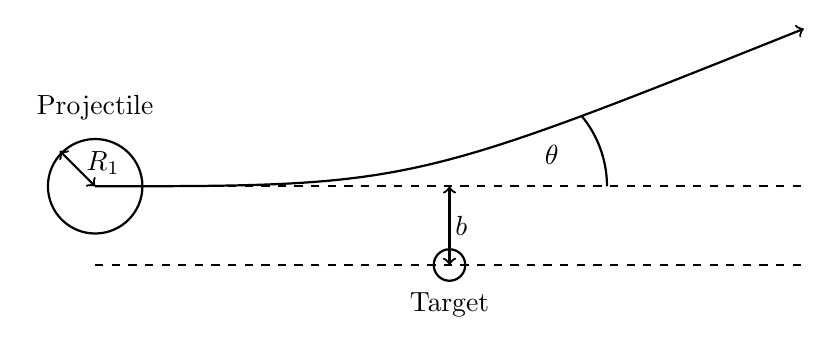
\begin{tikzpicture}
%    \draw[orange,thin] (0.0,0.0) grid (16.0,9.0);

    \draw[->,thick] (2,2) .. controls (6.0,2) .. (11,4);

%    \node [rotate=0,align=left]  at (10,2.7)    {Projected \\ trajectory};
    \draw[dashed,thick] (2,2) -- (11,2);


    \draw[black,thick] (2,2) circle (0.6);
        \draw[<->,thick] (2,2) -- (1.55,2.45);
    \node [rotate=0]  at (2.1,2.3)    {$R_1$};
    \node [rotate=0]  at (2.0,3.0)    {Projectile};
    \draw[<->,thick] (6.5,1) -- (6.5,2);

    % target
    \draw[black,thick] (6.5,1) circle (0.2);
    \draw[black,dashed,thick] (2,1) -- (11,1);
    \node [rotate=0]  at (6.5,0.5)    {Target};
%   \node [rotate=0]  at (6.95,1.1)    {$R_2$};
   \node [rotate=0]  at (6.65,1.5)    {$b$};

   % angle
    \draw[black,thick] (8.5,2) arc (0:40:1.4);
    % \draw[black,dashed,thick] (11,4) -- (11,1);
   \node [rotate=0]  at (7.8,2.4)    {$\theta$};


  \end{tikzpicture}
  \caption{Schematic illustration of the impact parameter.}
  \label{pic:impact}
\end{figure}



\subsubsection{Multiple Coulomb Scattering}

Coulomb scattering occurs when the projectile is deviated from its trajectory while interacting with the coulomb field of the atoms in the collimator material~\cite{Beringer:1900zz}. 

Throughout the passage of the material, the particle can be repeatedly subject to small angular Coulomb scattering and so accumulate an angular deviation significantly larger than from the individual interactions. This process, referred to as Multiple Coulomb Scattering (MCS), can be quantified by the RMS scattering angle $\theta_0$ which is well-described the Moli\`{e}re formula~\cite{Beringer:1900zz}
\begin{align}
\theta_0 = \frac{13.6\,\text{MeV}}{\beta \, c \, p} \, Z \, \sqrt{\frac{\Delta s}{X_0}} \, \left[ 1 + 0.038 \, \ln \left( \frac{\Delta s}{X_0} \right) \right] \, ,
\end{align}
where $\Delta s$ is the distance the particle traversed inside the material and $X_0$ is the radiation length that is a characteristic quantity for the target material. 

The radiation length is accessible via tabulated data or by means of the approximated formula depending on the charge $Z_m$, nucleon number $A_m$ and density $\rho_m$ of the target material~\cite{Beringer:1900zz}
%
\begin{align}
  X_0 = \frac{716.4 \, \text{g} \, \text{cm}^{-2} \, A_m}{\rho_m \, Z_m (Z_m+1) \, \ln (287/\sqrt{Z_m})} \, .
\end{align}
%
The radiation length for the most important collimator materials is given in \tabref{tab:radiation_lengths}.

\begin{table}[t]
\centering
\caption{Properties of the most important collimator materials, including materials foreseen for upgrades of the LHC collimation system. Data taken from~\cite{IPAC15:TUPTY029}.}
\label{tab:radiation_lengths}
\begin{tabular}{lllll}
\toprule
Material & $Z_m$ & $A_m$  & $\rho_m$ {[}g/cm$^3${]} & $X_0$ {[}cm{]}  \\ \midrule
C (CFC)  & 6     & 12.01  & 1.67                    & 25.57          \\
Cu       & 29    & 63.55  & 8.96                    & 1.435          \\
W        & 74    & 183.85 & 19.30                    & 0.35           \\
Mo$_2$C  & 30    & 67.978 & 8.40                     & 1.222         \\ \bottomrule
\end{tabular}
\end{table}

% DATA FROM ELENA FOR FAST IMPLEMENTATION IF NECESSARY
%       element Z       A       rho   X0[g/cm2] X0[cm] 
% 1	Be	4	9.01	1.848	65.19	35.276
% 2	Al	13	26.98	2.7	24.01	8.893
% 3	Cu	29	63.55	8.96	12.86	1.435
% 4	W	74	183.85	19.3	6.76	0.350
% 5	Pb	82	207.19	11.35	6.37	0.561
% 6	C (CFC)	6	12.01	1.67	-	25.57
% 7	C2	6	12.01	4.52	-	9.40
% -	graphite	6	12.01	2.25	42.700	18.978
% -	diamond	6	12.01	3.14	42.700	13.599
% -	B	5	10.8	2.37	52.690	22.232
% -	Ni	28	58.69	8.9	12.680	1.425
% 	O	8	16	-	34.240	-
% -	Al2O3	10	20.392	3.97	27.940	7.038
% 10	Mo	42	95.962	10.22	9.8	0.9589041096
% -	Mo2C	30	67.978	8.4	10.266	1.222
% 8	MoGr	6.653	13.532	2.5	29.828	11.931
% 9	CuCD	11.898	25.238	5.4	17.073	3.162
% 11	Glidcop	28.823	63.149	8.93	12.881	1.442
% 12	Inermet	67.657	166.677	18	6.922	0.385


\subsubsection{Energy Loss from Ionization}

  \begin{figure}[b]
  \centering
  \includegraphics[width=0.85\textwidth]{pictures/15091401.png}
  \caption{Stopping power as described by the Bethe-Bloch formula~\cite{Beringer:1900zz}. Compared to \eqref{eq:bethe}, the mean energy loss per traversed length is normalized by the density of the material.}  
  \label{pic:15091401}
  %/home/phermes/Desktop/lec1.png
  \end{figure}

Particles at the passage through matter can interact inelastically with the electrons of the atoms constituing the target material. At such encounters, a fraction of the projectile's kinetic energy is disposed into the energy required to deliberate an electron from an atom of the target material.

Quantitatively, the mean energy loss per traversed length unit in the material is described by the Bethe-Bloch formula~\cite{Beringer:1900zz}:
\begin{align}
- \left\langle\frac{dE}{dx}\right\rangle = \frac{4 \pi}{m_e c^2} \cdot \frac{nq^2}{\beta^2} \cdot \left(\frac{e}{4\pi\varepsilon_0}\right)^2 \cdot \left[\ln \left(\frac{2 \, m_e c^2 \, \beta^2}{I \cdot (1-\beta^2)}\right) - \beta^2\right] \, , \label{eq:bethe}
\end{align}
where $I$ is the mean excitation energy (which is tabulated for different materials), $m_e$ is the electron rest mass and $n$ is the electron density in the material.


The average energy loss depends on the projectile mass and velocity and on the atomic density of the target. The energy loss is shown as a function of $\beta \gamma$ and the particle type in \figref{pic:15091401}.

\subsubsection{Electromagnetic Dissociation} \label{chap:emd}
Electromagnetic dissociation (EMD) is a photonuclear reaction that occurs at ultraperipherical collisions of the involved nuclei \mbox{($b>R_1 + R_2$)}. The Lorentz contracted electric fields lead to the exchange of a large number of virtual photons which can induce the nuclear excitation of one or both of the involved nuclei~\cite{PhysRevSTAB17021006}. The cross section of the EMD process scales logaritmically with the relativistic $\gamma$ factor of the impacting nucleus~\cite{PhysRevSTAB17021006}. The excited nuclei dissipate the energy under the emission of one or more nucleons, where the emission of neutrons has the largest cross section for heavy nuclei such as \lead. An important example for the electromagnetic dissociation of this isotope is the production of $^{207}$Pb$^{82+}$ in the carbon material of the primary collimators 
\begin{align}
^{208}\text{Pb}^{82+} &+ ^{12}\text{C} \rightarrow ^{207}\text{Pb}^{82+}  + ^{12}\text{C} + n \, .
\end{align}
The residual heavy ion can again be subject to EMD, resulting in $^{206}$Pb$^{82+}$, a main contributor to the ion losses in the aperture of the LHC arcs, as discussed in \chapref{chap:STIER:full}. Overall, the EMD process is very important to consider in the picture of heavy-ion collimation, because the residual ions have rigidities very close to the main beam. They can travel through the magnetic lattice of the LHC over large distances and may cause distinct losses at given LHC elements. 

\subsubsection{Nuclear Interactions}
Nuclear encounters with impact parameters smaller or equal than the sum of the radii of the involved nuclei can lead to interactions over strong force. Whereas the reaction channel is similar to photonuclear interaction, with nuclear excitation of either the target or the projectile and their subsequent disintegration, the spectrum of residual nuclei is much wider when the particle has undergone a nuclear interaction~\cite{bartke:relativistic}. 

Typically residual ion fragments can cover the full isotope spectrum and therefore produce particles with rigidities far from the main beam. For the materials used in primary LHC collimators nuclear interactions occur with cross sections one order of magnitude above the one for EMD processes (see \tabref{tab:xsections} for a comparison) making them an important component in the study of loss patterns of heavy-ion collimaton debris.

Processes of fragmentation, either from EMD or nuclear interactions, come along with deviations in angle and transfer of transverse and longitudinal momentum. The created fragments thus populate not only a wide spectrum in terms of mass and charge, but also of angular coordinate (which can be superior to angular scattering from MCS) and momentum, which leads to additional glazing of the distribution of magnetic rigidities~\cite{PhysRevSTAB17021006}.

\begin{table}[h]
\caption{Cross sections for EMD and nuclear interactions of \lead ions for different fixed target materials at the 2011 LHC energy of $3.5\,Z\,$TeV and its design energy $7.0\,Z\,$TeV~\cite{PhysRevSTAB17021006}.}
\label{tab:xsections}
\centering
\begin{tabular}{ccccc}
  \toprule
       & \multicolumn{2}{c}{\begin{tabular}[c]{@{}c@{}}$\sigma$ {[}b{]}\\ $3.5\,Z\,$TeV\end{tabular}} & \multicolumn{2}{c}{\begin{tabular}[c]{@{}c@{}}$\sigma$ {[}b{]} \\ $7.0\,Z\,$TeV\end{tabular}} \\ \midrule
Target & EMD                                            & Nuclear                                         & EMD                                            & Nuclear                                         \\ \midrule
C      & 0.471                                          & 3.24                                            & 0.498                                          & 3.26                                            \\
Cu     & 10.16                                          & 5.09                                            & 11.05                                          & 5.11                                            \\
W      & 63.52                                          & 6.92                                            & 68.91                                          & 6.95   \\ \bottomrule                                         
\end{tabular}
\end{table}
 

\subsubsection{Nuclear Evaporation and Statistical Fragmentation}

The residual heavy ions generated at a cascade of interactions of either nature may still be in a nuclear charge state above the ground level. Depending on the mass of the fragment two physical processes of energy dissipation can be distiguished. 

Heavy nuclei can decay into their ground state by either nuclear fission, the emission of nucleons or $\gamma$ rays, a process referred to as nuclear evaporation~\cite{HEP2003:MOMT005}. Proton emission from nuclear evaporation is suppressed as compared to neutron emission because of the Coulomb barrier~\cite{HEP2003:MOMT005}.

Light residual ions are subject to fragmentation which can be statistically described by the Fermi breakup model~\cite{fermi:breakup}. In this model, significant momentum can be transferred to the fragments originating from this process.



\begin{table}[htbp]
\caption{Characteristic quantities for the most imporant physical processes of protons and lead ions traversing CFC at 7$\,Z\,$TeV. SCALED with DENSITY. CHECK IF CORRECT. Data partly taken from \cite{ICOSIMref02}.}
\begin{center}
\begin{tabular}{ c c c c }
\toprule
Physics Process & Unit & Proton & \lead \\ \midrule
$- \frac{dE}{E\,\mathrm{d}x}$ & [$10^{-5}$\,m$^{-1}$] & 11 & 917 \\ 
$\theta_\text{MCS}$ &  [$\,\mu$rad/$\sqrt{m}$] & 4.0 & 4.0 \\ 
Nuclear interaction length & [cm] & 47.9 & 3.1 \\ 
EMD length & [cm] & - & 23.9 \\ \bottomrule
\end{tabular}
\end{center}
\label{tab:physics_ions_matter}
\end{table}



\chapter{Simulation Tools}

Important contributions to the excellent performance of the LHC came from theoretical simulations. Many tools have been developed and used to predict various physics aspects of the machine. For collimation, particularly software for particle tracking and simulations of particle-matter interaction are important. The prior requires also a detailed model for optics computation, as the configuration of the magnetic lattice is crucial for the particle motion in the machine. In order to have a complete picture of the collimation efficiency, information must be exchanged between the tracking tool and the particle-matter interaction, which can be realized in different manners. In this chapter, different software tools important for the development of the heavy-ion collimation simulation tools are presented.



\section{MAD-X}
MAD-X (Methodical Accelerator Design)~\cite{MADXref01} is the standard tool to simulate beam dynamics and compute beam optics in particle accelerators. The software is a complete migration of MAD-8 (written in FORTRAN77) to C++ and was introduced in 2002 for the design and simulation of the LHC optics~\cite{MADXref02}.

The software computes the global Twiss parameters by means of transfer matrices for the individual lattice elements. The structure of the machine and the strengths of the magnets are given by the user by means of dedicated input files. A matching function provides the functionality to adjust specific variables such that previously defined constraints are fulfilled. An aperture model of the machine can be processed and compared with the beam position and dimensions to evaluate the available normalized aperture throughout the machine. A dedicated function produces the required optics input for SixTrack (see next Chapter). 



% ----------------------------------- PARTICLE MATTER INTERACTION ----------------------------------

\section{FLUKA}


\begin{figure}[t]  
    \centering
    \includegraphics[width=0.8\textwidth]{pictures/16060102.pdf}
    \caption{FLUKA geometry of the three primary collimators in IR7 for B1~\cite{skordis_fluka_model}.}  
    \label{pic:16031201}
    %/home/phermes/Dropbox/PhD/pictures/160601_fluka_collimators/annotated/coooo_annotated.pdf
\end{figure}


FLUKA (FLuktuierende KAskade) is a fully integrated Monte-Carlo package to simulate particle transport and the interaction of particles with matter~\cite{ferrari2005fluka}. The package simulates the interaction with the nuclei of the traversed material and particles generated in electromagnetic or hadronic cascades are kept track of. The software uses regularly updated physics models derived from experimental data and is used for a variety of simulations, including particle shower simulations and energy deposition studies. 

The species, energy and direction of the incident particles are given by the user in a dedicated input file. The geometry can be defined manually with a dedicated synthax or generated from the FLUKA element database (fedb) which contains LHC elements which may be assembled. The full geometry of the different LHC inserstion regions (see \chapref{}), is available as a FLUKA model and is regularly used to study energy deposition, activation or shower propagation for different beam loss scenarios. As an example, the geometry of three primary LHC collimators, including their mounting plates, is shown in \figref{pic:16031201}.

The FLUKA user input file is a sequence of command lines (called \textit{cards}), which define the simulation setup via different available options~\cite{}. The required output information can be selected, post-processed and written to dedicated files via 38 different user routines that can be linked to the FLUKA executable. Each user routine consists of FORTRAN code that can be adjusted to the specific requirements of the user. The options for pre-defined output can be set in the FLUKA input file by means of the respective card linked to a specific user routine. 


\section{SixTrack}

\subsection{Description}

\begin{figure}[b]
  \centering
  \includegraphics[width=1\textwidth]{pictures/15070701.png}
  \caption{BeamLossPattern algorithm to identify aperture losses SixTrack simulated particle tracks [S. Redaelli, R. Assmann, and G. Robert-Demolaize. Lhc aperture and commissioning
of the collimation system. Proceedings of the LHC Project Workshop
Chamonix XIV, 2005.].}  
  \label{pic:15070701}
  %/home/phermes/Desktop/tra.png
\end{figure}

SixTrack~\cite{SixTrackref01,SixTrackref02,SixTrackref03,SixTrackref04} is designed to provide symplectic six-dimensional tracking of relativistic proton beams in high energy synchrotrons over many turns. Initially developed for dynamic aperture studies, the software is subject to regular updates providing new features for dedicated functions or improved physics models. An important extension is the integrated routine for the simulation of proton collimation in high energy colliders as the LHC~\cite{1591725,collsixtrack}. \

The tracking algorithm is based on symplectic transfer maps derived from the accelerator Hamiltonian, which are implemented in both thick lens model and thin lens approximation~\cite{}. Based on these tracking maps, the array [$x,x',y,y',\sigma,p_\sigma,P$] is transported through the magnetic lattice of the accelerator. The symplecticity makes SixTrack an excellent tool to provide accurate tracking over a large number of turns. 

The collimation subroutine provides an integrated environment for 6D tracking together with a Monte-Carlo Module to simulate the interaction of the protons with the material of the collimation devices. For this purpose, physics models and cross-sections for different types of interactions are implemented for different collimator materials. The SixTrack particle-matter interaction simulation includes energy loss via ionization, multiple Coulomb scattering, and nuclear interactions at the passage of the protons through the collimator. 

In order to identify the loss distribution in the ring, the individual particle tracks are compared to a detailed model of the LHC aperture. If the track of a beam particle is identified to intercept the aperture, the loss location is identified with a precision of 0.1~m and the information is saved in a dedicated output file. The aperture check is first carried out at dedicated aperture markers to reduce the required computing time. Beginning from the marker, particle track is then reversely extrapolated as a straight line and the aperture check is iteratively repeated in steps of $10\,$cm (see \figref{pic:15070701}) until the loss location is indentified.  

In the current SixTrack release version~\footnote{SixTrack Version 4.5.34 from 20.04.2016}, this algorithm is executed on a post-processing level by means of the software BeamLossPattern~\cite{}. Given that all particle tracks have to be saved and analyzed in this approach, this method of loss detection is very time- and space-consuming. A recently developped on-line aperture check~\cite{} compares the simulated proton tracks to the aperture at each tracking step, making the extraction of the particle tracks unnecessary.  

Protons interacting with the collimators are considered to be lost if they undergo nuclear inelastic scattering. A significant amount of losses in the aperture arises from protons having undergone single diffractive scattering. In this process, the proton interacts with a nucleus of the collimator material and is excited to a higher nuclear state. This excited state decays into a proton and other particles and the energy of the outgoing proton is reduced with respect to the incident proton~\cite{}. 

\subsection{Simulation Setup and Running of Collimation SixTrack}
The SixTrack options and input is given via two dedicated input files
\begin{itemize}
  \item fort.2: defining the optical configuration of the accelerator. This file can be automatically generated from MAD-X.
  \item fort.3: Selection of options and beam settings. The most relevant options for collimation studies are the number of tracked particles, number of turns through the machine, particle energy, RF settings, collimator settings and initial distribution. 
\end{itemize}
The COLLIMATION block in the fort.3 file contains information about the settings of the different collimator families. The latter are defined by a collimator database input file, containing information on the name, length and material of the different collimators. The classification of the collimator family is conducted by the prefix of the collimator name and the region where the collimator is installed. 

The initial beam halo can be selected from different options, the most notable ones being an annular halo in $x,x'$ at an amplitude large enough such that the particles hit the primary collimator, or a pencil beam with controlled impact parameter at a given collimator. Even though 

Collimation simulations with SixTrack are usually carried out for 200 turns with an initial sample of 6.4 million protons  starting at IP1. Given the large amount of required space which has to be allocated for the aperture loss detection, and the high amount of required CPU time, the simulations are split into 1000 sub-simulations which are submitted to the CERN batch computing service in which they are processed in parallel, if possible~\cite{}[http://information-technology.web.cern.ch/services/batch]. The post-processing is carried out on the virtual machine of the cluster, such that only the relevant output is saved back in the user directory and the required disk space is reduced by several orders of magnitude. 

% \section{ICOSIM}

% ICOSIM (Ion Collimation Simulation)~\cite{ICOSIMref02,ICOSIMref01} is a tool to simulate the cleaning performance of the collimation system with heavy-ion beams. The tool, which is implemented in Matlab, was developed to evaluate the efficiency of the LHC cleaning system for heavy ions before the start of the LHC.
% It is an integrated program for particle tracking with a Monte-Carlo module to simulate the interaction of heavy-ions with the collimator materials. The tracking routine is based on a matrix multiplication with chromatic modelling in linear approximation and sextupole fields in thin-lens approximation. The information about the magnetic lattice is read from MAD-X output. Along with the tracking, the particle amplitudes are compared to a simplified aperture model, in which the aperture cross sections are approximated by an ellipse. Once the aperture is identified to be intercepted at the end of an element, the exact location is determined by extrapolation, as desribed in the previous chapter. 

% The integrated Monte-Carlo module simulates the interaction of the ions with matter, including energy loss from ionization via the Bethe-Bloch equation and multiple Coulomb scattering, as well as fragmentation processes from EMD and NF~\cite{ICOSIMref02}. The latter is computed using tabulated cross-section information for the two processes which is generated beforehand with FLUKA. When a particle is subject to fragmentation in the collimator, the heaviest fragment is given back to the tracking routine, and transverse momentum transfers from the fragmentation process are not taken into account~\cite{ICOSIMref02}. 

% ICOSIM is equipped with a subroutine to sample the initial distribution, typically a Gaussian distribution in $x,x'$. In order to simulate diffusion, the emittance of the tracked particle bunch is increased by applying random transverse kicks. The simulation is typically carried out over 500 turns for 2 million initial particles. 

\section{SixTrack-FLUKA Coupling}

\begin{figure}[b]  
    \centering
    \includegraphics[width=0.65\textwidth]{pictures/16060101.pdf}
    \caption{Principle of the SixTrack-FLUKA coupling. At every collimator extraction marker (red) the particle bunch is sent to FLUKA where the interaction with the collimator is simulated. The resulting distribution is then re-injected in SixTrack at the injection marker (green), from where the tracking is continued.}  
    \label{pic:16060101}
    %/home/phermes/Dropbox/PhD/pictures/160601_six_fluka_coupling/test/annotated/drawing_annotated.pdf
\end{figure}


The SixTrack-FLUKA online coupling~\cite{mereghetti_ipac2013_1} is a dedicated framework in which the two simulation codes SixTrack and FLUKA are ran in parallel to simulate the cleaning performance of the collimation system by complementary tracking and particle-matter interaction at the collimators. This approach was developed to combine the advantages of both codes with their detailed and regularly updated physics models. The backbone of the particle exchange is a network port which transfers particle information between the two codes while both of them keep running in the background. This shortens the time required normally for subsequent simulations because each code does not have to be re-initialized after each particle exchange and post-processing of data becomes unnecessary. 


\begin{figure}[htbp]
  \centering
  \begin{tikzpicture}
    \node[anchor=south west,inner sep=0] (image) at (0,0) {\includegraphics[width=1.0\linewidth]{pictures/16070701.png}};
    %\node [draw,rotate=90,x={(image.south east)},y={(image.north west)}]                   at (0.50,0.50)    {text0};
    %\node [draw,rotate=0 ,x={(image.south east)},y={(image.north west)}]                   at (0.22,0.96)    {text1};
    %\node [draw,rotate=0 ,x={(image.south east)},y={(image.north west)},anchor=west]       at (0.22,0.80)    {text2};
    %\draw[->,color=black,thick,x={(image.south east)},y={(image.north west)}]             (0.42,0.22) -- (0.37,0.23);
  \end{tikzpicture}
  \caption{Collimator models in the FLUKA input file used for the SixTrack-FLUKA coupling.}  
  \label{pic:16070701}
  %/afs/cern.ch/work/p/phermes/private/150629_coupling_ions/hiSix/160315_HLLHC//home/phermes/Desktop/fedb.png
  \end{figure}



The basic principle of the SixTrack-FLUKA coupling is illustrated in \figref{pic:16060101}. The magnetic lattice used in SixTrack is expanded by additional collimator extraction markers at which SixTrack sends the particle distribution to FLUKA, where the interaction with the collimator is simulated. Conversely, at the end of the collimator, the distribution of residual particles is sent back to SixTrack and re-injected into the lattice at a dedicated injection marker from which the tracking is continued. 

The marker locations correspond to the beginning and end of the collimator tanks. The FEDB stores detailed models of each collimator type (see \figref{pic:16070701}) and the settings of the individual collimators are applied in a dediacted pre-processing algorithm in which the FLUKA input file, required for the coupling simulation, is produced. Every collimator is assigned to a collimator ID. Residual protons which are not identical to the incoming protons (e.g. those produced in nuclear interactions) are assigned to a new particle ID, which can take values up to 2000. 

An important feature required for collimation studies in this framework is an on-line aperture check during the tracking instead of computing the aperture losses on a post-processing level as done in the nominal collimation SixTrack algorithm. Such an on-line aperture check was implemented in 2014. With this algorithm SixTrack continuously compares the particle coordinates to a detailed model of the LHC aperture. With the initial aperture check carried out at the markers, the losses can be more precisely localized by backwards extrapolation, similarly to the aperture check with \texttt{BeamLossPattern}, providing a full comparability of the loss maps generated in collimation SixTrack and with the coupling.

The framework allows for the automatic output of a \texttt{toucMap} file which contains information on the impact position at every collimator. This data can be subsequently used for the detailed shower propagation simulations in FLUKA. With this type of simulation the energy deposited in the regions downstream of the collimators can be calculated by taking into account the contribution of all secondary shower particles. The interaction of the shower particles with the LHC hardware is precisely computed to determine the energy deposited in them. Furthermore, the shower simulations can be used to quantiatively predict the resulting BLM signals. Compared to the nominal cleaning simulations with SixTrack these simulations are extensive in terms of time and space consumptions and are therefore rather carried out for dedicated configurations, e.g. when experimentally measured quench limits shall be theoretically accessed.

